% TSD 2013 template for camera-ready version
%
% v. 2013-05-20 by Ivan Habernal (habernal@kiv.zcu.cz)
%
% Based on Springer LNCS series template.
\documentclass[runningheads,a4paper]{llncs}

\usepackage{times}
\usepackage{amssymb}
\setcounter{tocdepth}{3}
\usepackage{graphicx}
\usepackage{url}

% TSD 2013: Add any additional packages you use in your manuscript
% -----pack
% \usepackage{xxx}

\usepackage[utf8]{inputenc}
\usepackage[english]{babel}
\usepackage[T1]{fontenc}
\usepackage{textcomp}
\usepackage{multirow} 
\usepackage{siunitx}

% -----

% TSD 2013: Add your custom definitions etc., if required
% -----misc
% \newcommand{\xxx}[1]{[#1]}
% -----


\newcommand{\keywords}[1]{\par\addvspace\baselineskip
\noindent\keywordname\enspace\ignorespaces#1}

% TSD2013: Put your e-mail addresses here
\urldef{\mailsa}\path|{luiza.orosanu, denis.jouvet}@loria.fr|
%\urldef{\mailsc}\path|other_mails_if_needed|    

\begin{document}

% TSD2013: Put your title here (please, use capitalization, see e.g.
% http://en.wikibooks.org/wiki/Basic_Book_Design/Capitalizing_Words_in_Titles)
\title{Comparison and Analysis of Several Phonetic Decoding Approaches}

% TSD 2013: a short form should be given in case the title is too long for the running head
\titlerunning{Comparison and Analysis of Several Phonetic Decoding Approaches}

% TSD 2013: Author's names. Chinese authors should write their first names(s)
% in front of their surnames. This ensures that the names appear correctly in
% the running heads and the author index.
% If the names contain accented characters, please use escape codes
% (refer to http://en.wikibooks.org/wiki/LaTeX/Special_Characters#Escaped_codes)
\author{Luiza Orosanu \inst{1,2,3}  \and Denis Jouvet \inst{1,2,3}}

% TSD 2013: For authors from different institutions, please use the following
% form including institution reference
% \author{Firstname1 Surname1\inst{1} \and Firstname2 Surname2 \inst{2}}

% TSD 2013: Author's names for headings. For 1-2 authors, use the following form
\authorrunning{Luiza Orosanu and Denis Jouvet}
% TSD 2013: For more than 2 authors, please, use the following
% \authorrunning{Name1 Surname1 et al.}

% TSD 2013: The authors' affiliations
\institute{Speech Group, LORIA\\
\inst{1} Inria, Villers-lès-Nancy, F-54600, France \\
\inst{2} Université de Lorraine, LORIA, UMR 7503, Villers-lès-Nancy, F-54600, France \\
\inst{3} CNRS, LORIA, UMR 7503, Villers-lès-Nancy, F-54600, France \\
\mailsa\\
}

% TSD 2013: Put all authors' names to the proceeding index (surname, first name)
\index{Orosanu, Luiza}
\index{Jouvet, Denis}

\toctitle{} \tocauthor{}

\maketitle


\begin{abstract}
% TSD 2013:
This article analyzes the phonetic decoding performance obtained with different choices of linguistic units. The context is to later
use such an approach as a support for helping communication with deaf people, and to run it on an embedded decoder on a portable terminal,
which introduces constrains on the model size. As a first step, this paper compares the performance of various approaches on the ESTER2 and
ETAPE speech corpora. Two baseline systems are considered, one relying on a large vocabulary speech recognizer, and another one relying
on a phonetic n-gram language model. The third model which relies on a syllable-based lexicon and a trigram language model, provides a good
tradeoff between model size and phonetic decoding performance. The phone error rate is only 4\% worse (absolute) than the phone error rate
obtained with the large vocabulary recognizer, and much better than the phone error rate obtained with the phone n-gram language model. Phone
error rates are then analyzed with respect to SNR and speaking rate. 
% TSD 2013: keywords, comma-separated
\keywords{syllables, deaf, speech recognition, embedded system}
\end{abstract}


\section{Introduction}

Support for deaf people or for people with hearing impairment is an
application area of automatic speech processing technologies \cite{TSD1}.
Their objective is to become a communication aid for disabled persons.
Over the past decades, scientists have tried to offer a better speech
understanding, by displaying phonetic features to help lipreading
\cite{TSD2}, by displaying signs in sign language through an avatar
\cite{TSD3}, and of course by displaying subtitles, generated in
a semi-automatic or fully automatic manner. The ergonomic aspects
and the conditions for using speech recognition to help deaf people
were analyzed in \cite{TSD4}. One of the main drawbacks of speech
recognition systems is their incapacity of recognizing the words that
do not belong to their vocabulary. Given the limited amount of speech
training data, it is impossible to conceive a system that covers all
the words, let alone the proper names or abbreviations. Furthermore,
recognition systems are not perfect, it happens quite frequently that
a word is confused with another one which is pronounced the same (homophone)
or almost the same. The performance is very far from human performance
\cite{TSD5} and even degrades rapidly in the presence of noise. Therefore,
in the context of communication aids for deaf people, displaying the
orthographic form of the recognized words may not be an ideal solution. 

IBM has thus tested subtitling the phonetic speech of a speaker, with
the system called LIPCOM \cite{TSD6}. The application was based on
a phonetic decoding (with no prior defined vocabulary) and the result
was displayed as phonemes coded on one or two letters. More recent
studies have measured the contribution of confidence measures \cite{TSD7}
within the use of automatic transcription for deaf people \cite{TSD8}.
Subjective tests have shown a preference for displaying the phonetic
form of the words with a low confidence score. 

An alternative solution is to use multi-phone sub-word units, like
the syllable. Its appeal lies in its close connection to human speech
perception and articulation, since it's more intuitive for representing
speech sounds. The use of syllable-size acoustic units in speech recognition
has been investigated in the past \cite{TSD9,TSD10}, for large vocabulary
continuous speech recognition (usually in combination with context
dependent phones) \cite{TSD11,TSD12} or for phonetic decoding only
\cite{TSD13}. In this last case \cite{TSD13}, because of the structure
of the acoustic units, coarticulation was modeled between phonemes
inside the syllable unit, but no context-dependent modeling was taken
into account between syllable units, moreover the language model applied
at the syllable level was a bigram. Besides, to overcome the limited
size of any speech recognizer lexicon, studies have been conducted
in extending the word-based lexicon with fragments, typically sequences
of phonemes determined in a data driven way; this extension helped
providing better acoustic matches on out-of-vocabulary portions of
the speech signal, which globally led to a smaller phonetic error
rate \cite{TSD14}. 

In this paper we shall investigate the use of syllables at the lexical
level. The syllables are described in terms of phonemes, which are modeled 
with context-dependent 3-states HMM. The language model applied on the syllables 
is a trigram. We have followed the rules proposed in a recent study for 
detecting syllables boundaries within a sequence of phonemes \cite{TSD15}. 
These rules are used to derive the syllables from the phonetic forced-aligned training
data, and some criteria are applied to reduce the list of syllables
constituting the lexicon. Performance is reported in terms of phoneme
error rate, and evaluations are conducted on two large French speech
corpus. 

The work presented in this paper is part of the RAPSODIE project, 
which aims at studying, deepening and enriching the
extraction of relevant speech information, in order to support
communication with deaf or hard of hearing people. Therefore,
the optimal solution should determine the best compromise for
the recognition model and the best way of presenting the recognized
information (words, syllables, phonemes or combinations),
within the constraints of limited available resources (the
memory size and computational power of an embedded system).

The paper is organized as follows. The first section
provides a description of the various linguistic units used in our
analysis, that is phonemes, syllables and words. The second part of the paper
is devoted to the description of experiments and the discussion of results. 
The different approaches, based on phoneme, syllable and word units, are compared 
on the ESTER and ETAPE data. Then, a detailed analysis of the performance is carried 
out with respect to signal-to-noise ratio (SNR) and speaking rate.


\section{Linguistic units}

This section describes the linguistic units used in our analysis:
the phonemes, as the basic and smallest linguistic unit, the syllables,
as the phonological ``building blocks'' of words,
and the words, as the largest linguistic unit, but at the same time
the smallest linguistic element which caries a real meaning. Note
that the choice of linguistic units impacts on the language model. 
In the experiments reported later, the acoustic unit is always the phoneme
and the language models are always trigram statistical models.


\subsection{Phonemes}

Regarding the pronunciation lexicon, the pronunciation of a phoneme
is the phoneme itself. Using this type of linguistic unit, we minimize
the size of our vocabulary (less than 40 phonemes for the French language)
and therefore the size of our language model. But unfortunately, with
less modeling power usually comes worse performance.


\subsection{Words}

The word lexicon contains the mappings from words to their pronunciations
in the given phoneme set. Given that French is a non-phonetic language,
some letters can be pronounced in different ways or sometimes not
at all, and a normally silent consonant at the end of a word can be
pronounced at the beginning of the word that follows it (``liaison'').
So, in order to make the automatic phonetic transcription as fluid
as the real speech, the dictionary usually contains several pronunciation
variants for each word. Using words as linguistic units leads to
a large vocabulary (about 97,000 words in our dictionary) and therefore
also to a large language model. This kind of model usually gives the
best performance, but with the cost of large memory use and slow computational
time (hence, not ideal for embedded systems).


\subsection{Syllables}

Regarding the vocabulary, the pronunciation of a ``phonetic'' syllable is its
decomposition into the phonemic components. In order to account for the ``liaison''
events, the words are not processed individually. The training corpora is
entirely phonetized and the resulting continuous list of phonemes
is processed by the syllabification tool. The phonetization process
is realized by force-aligning the manual transcriptions. Note that
a word can have several pronunciation variants, and that one or more
phonemes might be missing in some of them. Our syllabification tool
is based on the rules described in \cite{TSD15}, which follow two
main principles: a syllable contains a single vowel and a pause designates
a syllable's boundary. Therefore, the syllabification algorithm will
give out a list of syllables and pseudo-syllables. The pseudo-syllables
are the units where one vowel is surrounded by a large number of consonants,
which normally should not belong to a single syllable. In order to
filter some of the pseudo-syllable models, we have chosen to create
different lists corresponding to two criteria : a minimum number of
occurrences within the training corpora, and a maximum number of phonemes
per syllable. The number of linguistic units of each list varies between
4,000 (maximum 3 phonemes, minimum 10 occurrences) and 16,000 (minimum
1 occurrence). Using syllables as linguistic units leads to a compromise
between the memory use and computational time (ideal for embedded systems).


\section{Experiments and results}

This section describes the data sets and tools used in our experiments,
along with the corresponding results.


\subsection{Data}

The speech corpora used in our experiments come from the ESTER2 \cite{TSD16}
and the ETAPE \cite{TSD17} evaluation campaigns, and the EPAC \cite{TSD18}
project. The ESTER2 and EPAC data are French broadcast news collected
from various radio channels, thus they contain prepared speech, plus
interviews. A large part of the speech data is of studio quality,
and some parts are of telephone quality. On the opposite, the ETAPE
data correspond to debates collected from various radio and TV channels.
Thus this is mainly spontaneous speech. The speech data of the ESTER2
and ETAPE train sets, as well as the transcribed data from the EPAC
corpus, were used to train the acoustic models. The training data
amounts to almost 300 hours of signal and almost 4 million running
words. The phoneme-based language model and the syllable-based language
models were also trained on the results of the forced-alignments of ESTER2, 
ETAPE and EPAC corpora, on about 12 million running phonemes and on about 6 million running
syllables. 

For the creation of the word-based language model, various text corpora
were used: more than 500 million words of newspaper data from 1987
to 2007; several million words from transcriptions of various radio
broadcast shows; more than 800 million words from the French Gigaword
corpus \cite{TSD19} from 1994 to 2008; plus 300 million words of
web data collected in 2011 from various web sources, and thus mainly
covering recent years. For the word-based lexicon, the vocabulary
of about 97,000 words, was developed for the ETAPE evaluation campaign.
The pronunciation variants were extracted from the BDLEX lexicon \cite{TSD20}
and from in-house pronunciation lexicons, when available. For the
missing words, the pronunciation variants were automatically obtained
using JMM-based and CRF-based Grapheme-to-Phoneme converters \cite{TSD21}.


\subsection{Configuration}

The SRILM tools \cite{TSD22} were used to create the statistical
language models. The Sphinx3 tools \cite{TSD23} were used for training the acoustic models and for decoding the audio signals. The MFCC (Mel Frequency Cepstral Coefficients) acoustic
analysis computes 13 coefficients (MFCC and energy) every 10 ms. The acoustic HMM models were modeled with a 64 Gaussian mixture, and adapted to male and female data.


\subsection{Results}

The development sets of the ESTER2 (non-African radios, about 42,000 running words and 142,000 running phonemes) 
and ETAPE (entire set, about 82,000 running words and 263,000 running phonemes)
data are used in the experiments reported below.

The COALT (Comparing Automatic Labelling Tools) software \cite{TSD24}
was used for the analysis of results (phoneme error rates). The compared
files are the hypothesis .ctm file (resulting from the decoding process)
along with the reference .stm file. The CTM file consists of a concatenation
of time-marked phonemes. The STM (segment time marked) file describes
the reference transcript and consists of the results of the forced-alignment (sequences of phonemes). 

\begin{table}[ht]
\begin{center}
\caption{Characteristics of language models}
\begin{tabular}{|l|S[tabformat=3.1]|S[tabformat=3.2]|S[tabformat=3.2]|r|}
\hline
\multirow{2}{*}{\bf LM} & \multicolumn{3}{c|}{\bf \# of n-grams} & \multirow{2}{*}{\bf Size [MB]} 		\\ \cline{2-4}
 & {\bf n=1} & {\bf n=2} & {\bf n=3} & 		\\ \hline
{\bf phonemes} & \multicolumn{1}{r|}{40} & \multicolumn{1}{r|}{1347} & \multicolumn{1}{r|}{30898} & 0.21 	\\ \hline 
{\bf syl\_min4occ} & 8.3K & 0.38M & 1.73M & 9.97 								\\ \hline
{\bf words} & 97.3K & 43.35M & 79.30M & 1269.81 								\\ \hline
\end{tabular}
\label{Table-LMs}
\end{center}
\end{table}

Table \ref{Table-LMs} describes some of the language models (LM) used in our experiments.
With phoneme-based language model, the number of 3-grams is around
30,000 which leads to a minimum disk usage. With syllable-based language
model, the number of 3-grams is around 1.7 M (for the list of syllables
seen at least 4 times in the training data set) which leads to an
average disk usage. Using a large vocabulary, the number of 3-grams
is around 79.3 M which leads to the largest disk usage. 

\begin{table}[ht]
\begin{center}
\caption{Performance analysis on ETAPE and ESTER2 corpora [\%] }
\begin{tabular}{|l||S[tabformat=3.2]|S[tabformat=3.2]|S[tabformat=3.2]|S[tabformat=3.2]||S[tabformat=3.2]|S[tabformat=3.2]|S[tabformat=3.2]|S[tabformat=3.2]|}
\hline
\multirow{2}{*}{\bf LM} & \multicolumn{4}{c||}{\bf Results on ETAPE} & \multicolumn{4}{c|}{\bf Results on ESTER2} 	\\ \cline{2-9} 
 & {\bf PER} & {\bf Ins} & {\bf Del} & {\bf Sub} & {\bf PER} & {\bf Ins} & {\bf Del} & {\bf Sub} 			\\ \hline
{\bf phonemes} & 38.19 & 2.82 & 15.40 & 19.97 & 34.09 & 3.53 & 11.64 & 18.92 						\\ \hline
{\bf syl\_min4occ} & 22.05 & 3.34 & 8.50 & 10.21 & 16.13 & 3.94 & 4.88 & 7.31 						\\ \hline
{\bf words} & 18.21 & 3.11 & 8.01 & 7.09 & 12.44 & 3.41 & 4.62 & 4.40 							\\ \hline
\end{tabular}
\label{Tab:performance-ETAPE}
\end{center}
\end{table}

Table \ref{Tab:performance-ETAPE} presents some of the results obtained on the ETAPE and
ESTER2 development sets, described in terms of phoneme error rates (PER), along with their corresponding percentages 
of insertions (Ins), deletions (Del) and substitutions (Sub).
As expected, the best results were obtained with the large vocabulary recognizer. By using only the syllables
seen at least 4 times within the training data set, we limit the size
of the lexicon (about 8,000) and the size of the language model (only
about 10MB), and we achieve nevertheless good phonetic decoding performance.
The phone error rate is only 4\% worse (absolute) than the phone error
rate obtained with the large vocabulary recognizer, and much better
than the phone error rate obtained with the phone n-gram language
model. All the other syllable lists give more or less the same results.
Which means that starting with a minimum number of 7,000 linguistic
units we can achieve similar results as with the total number of $\sim$16,000
units. Given that ESTER2 contains mainly prepared speech and that
ETAPE contains mainly spontaneous speech, the results obtained on
ESTER2 are, as expected, better than the ones obtained on ETAPE. 

\begin{figure}[t!]
\begin{centering}
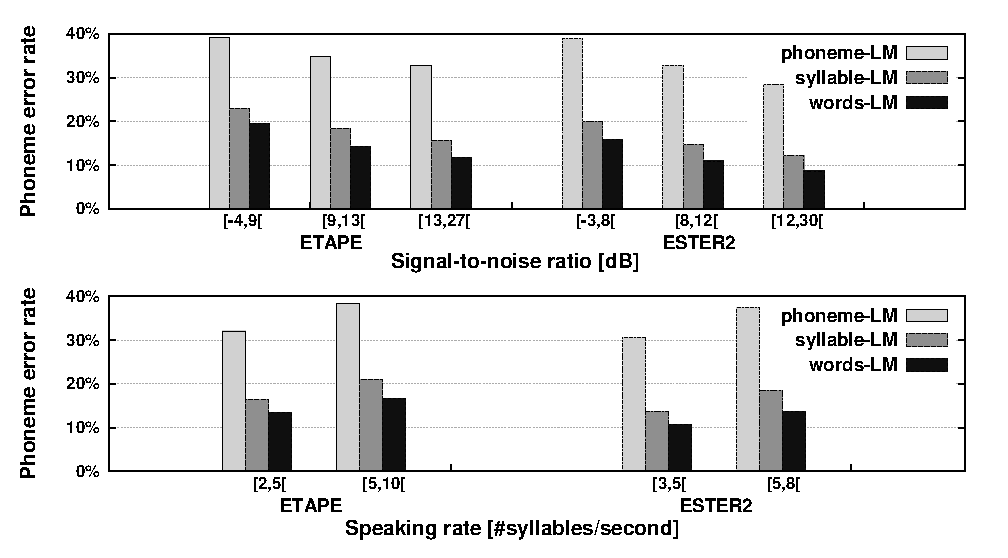
\includegraphics[scale=0.74]{Image/all}
\caption{ Analysis of the phoneme error rates on the ETAPE \textit{(left)} and ESTER2 \textit{(right)} corpora, with respect to signal-to-noise ratio \textit{(top)} and speaking-rate \textit{(bottom)} }
\label{Fig:stats}
\end{centering}
\end{figure}

\begin{equation}
SNR_{dB}=10log_{10}\frac{P_{signal}}{P_{noise}}\approxeq10\left(\frac{ln\left(\overline{C_{0}}_{vowel}\right)}{ln\left(10\right)}-\frac{ln\left(\overline{C_{0}}_{noise}\right)}{ln\left(10\right)}\right)
\label{eq:1}
\end{equation}

Figure \ref{Fig:stats} reports an analysis of the performance with respect to the SNR ratios and the speaking rates of both speech corpora, limited to speech segments longer than 5 seconds. We have observed that the performance improves when the SNR ratio increases and that the performance degrades when the speaking rate increases. The SNR values were obtained from the average values of the $C_{0}$ MFCC coefficients (as computed by \textit{sphinx\_fe} tool) of vowels relative to noise/silence, converted afterwards to dB (cf. eq. \ref{eq:1}). The speaking rates were computed as the number of vowels per second.

\begin{table}[ht]
\begin{center}
\caption{Analysis of the phone error rate(\%) on ETAPE \textit{(left)} and on ESTER2 \textit{(right)}, with respect to signal-to-noise ratios and speaking rates criteria}
\begin{tabular}{|S[tabformat=2,2]|S[tabformat=2.2]|S[tabformat=2.2]|}
\multicolumn{1}{c}{} & \multicolumn{2}{c}{\bf Speaking rate} 	\\ \cline{2-3}
\multicolumn{1}{c|}{\bf SNR} & {\bf [2,5[} & {\bf [5,10[} 	\\ \hline
\multicolumn{1}{|c|}{\bf [-4,9[} & 19.70 & 24.98 		\\ \hline
\multicolumn{1}{|c|}{\bf [9,13[} & 16.54 & 19.71	 	\\ \hline
\multicolumn{1}{|c|}{\bf [13,27[} & 13.74 & 17.28	 	\\ \hline
\end{tabular}
\hspace{1cm}
\begin{tabular}{|S[tabformat=2,2]|S[tabformat=2.2]|S[tabformat=2.2]|}
\multicolumn{1}{c}{} & \multicolumn{2}{c}{\bf Speaking rate} 	\\ \cline{2-3}
\multicolumn{1}{c|}{\bf SNR} & {\bf [3,5[} & {\bf [5,8[} 	\\ \hline
\multicolumn{1}{|c|}{\bf [-3,8[}  & 17.66 & 22.38 		\\ \hline
\multicolumn{1}{|c|}{\bf [8,12[}  & 12.17 & 17.76	 	\\ \hline
\multicolumn{1}{|c|}{\bf [12,30[} & 10.93 & 14.01	 	\\ \hline
\end{tabular}
\label{Tab:snr-vspeed}
\end{center}
\end{table}

Table \ref{Tab:snr-vspeed} presents the results obtained with the syllable language model on both corpora 
(speech segments longer than 5 seconds), with respect to both the SNR and the speaking rates criteria. 
We can naturally observe that the best results are obtained with the highest SNR ratio and the lowest 
speaking rate (less than five syllables per second). The results then degrade 
in both directions: when the SNR ratio decreases and when the speaking rate increases.


\section{Conclusions}

This paper presented a detailed study on the phonetic decoding performance
on two French speech corpora (ETAPE and ESTER2).
We were interested in finding the best compromise between computational
cost and usability of results, constrains that must be met in order
to be able to create an embedded speech recognition decoder on a portable
terminal. The context is to later use such an approach as a support
for helping communication with deaf people. Two baseline systems were
considered. The first one relies on a large vocabulary speech recognizer;
it gives the best results ($\sim$18\% phoneme error rate (PER) on
ETAPE and $\sim$12\% PER on ESTER2), but it uses a lot of memory
and computational power. The second one relies on a phonetic n-gram
language model; it does not use much memory, nor computational power,
but it does not give good results neither ($\sim$38\% PER on ETAPE
and $\sim$34\% PER on ESTER2). Then syllable language models were investigated. 
Keeping only the most frequent syllables leads to a limited-size lexicon and language
model, which nevertheless provides good phonetic decoding performance.
The phone error rate is only 4\% worse (absolute) than the phone error
rate obtained with the large vocabulary recognizer, and much better
than the phone error rate obtained with the phone n-gram language
model. Finally, a detailed analysis of the phoneme error rate was 
conducted with respect to SNR and speaking rate.

Future work will focus on the best, suitable way of presenting the
recognized information (phonemes, syllables, words or combinations),
based on relevant confidence measures, so that it maximizes communication
efficiency with deaf people.

\section{Acknowledgements}

The work presented in this article is part of the RAPSODIE project, and has received support from the “Conseil Régional de Lorraine” and from the “Région Lorraine” (FEDER) (http://erocca.com/rapsodie).


\begin{thebibliography}{1}

\bibitem[1]{TSD1} Schönbächler, J.: Le traitement de la parole pour les personnes handicapées. Travail de séminaire (2003)

\bibitem[2]{TSD2} Sokol, R.: Réseaux neuro-flous et reconnaissance de traits phonétiques pour l'aide à la lecture labiale. Thèse Université de Rennes (1996)

\bibitem[3]{TSD3}Cox, S., Lincoln, M., Tryggvason, J., Nakisa, M., Wells, M., Tutt, M. and Abbott, S.: Tessa, a system to aid communication with deaf people. Proceedings of the 5th international ACM conference on Assistive technologies, pp. 205-212 (2002)

\bibitem[4]{TSD4} Woodcock, K.: Ergonomics and automatic speech recognition applications for deaf and hard-of-hearing users. Technology and Disability, vol. 7, pp. 147-164 (1997)

\bibitem[5]{TSD5}Lippmann, R.: Speech recognition by machines and humans. Speech Communication, n\textdegree{} 22, pp. 1-15 (1997)

\bibitem[6]{TSD6}Coursant-Moreau, A. and Destombes, F.: LIPCOM, prototype d'aide automatique à la réception de la parole par les personnes sourdes. Glossa, n\textdegree{} 68, pp. 36-40 (1999)

\bibitem[7]{TSD7}Jiang, H.: Confidence measures for speech recognition: A survey. Speech Communication, vol. 45, n\textdegree{}4, pp. 455-470 (2005)

\bibitem[8]{TSD8}Razik, J., Mella, O., Fohr, D. and Haton, J.-P.: Transcription automatique pour malentendants: amélioration à l'aide de mesures de confiance locales. Journées d'Etude de la parole (2008)

\bibitem[9]{TSD9}Zhang, L. and Edmondson, W. H.: Speech recognition using syllable patterns. 7th International Conference on Spoken Language Processing (2002)

\bibitem[10]{TSD10}Tachbelie, M., Besacier, L. and Rossato, S.: Comparison of syllable and triphone based speech recognition for Amharic. Proceedings of the LTC, pp. 207\textendash{}211 (2011)

\bibitem[11]{TSD11} Ganapathiraju, A., Hamaker, J., Ordowski, M., Doddington, G. and Picone, J.: Syllable-based large vocabulary continuous speech recognition. IEEE Transactions on Speech and Audio Processing., vol. 9, n\textdegree{} 4, pp. 358\textendash{}366 (2001)

\bibitem[12]{TSD12} Hämäläinen, A., Boves, L. and de Veth, J.: Syllable-Length Acoustic Units in Large-Vocabulary Continuous Speech Recognition. Proceedings of SPECOM (2005)

\bibitem[13]{TSD13}Blouch, O., Collen, P.: Reconnaissance automatique de phonemes guide par les syllables. Journées d'Etude de la parole (2006)

\bibitem[14]{TSD14}Rastrow, A., Sethy, A., Ramabhadran, B. and Jelinek, F.: Towards using hybrid, word, and fragment units for vocabulary independent LVCSR systems. Proceedings Interspeech (2009)

\bibitem[15]{TSD15}Bigi, B., Meunier, C., Bertrand, R. and Nesterenko, I.: Annotation automatique en syllabes d\textquoteright{}un dialogue oral spontané. Journées d'Etude de la parole (2010)

\bibitem[16]{TSD16}Galliano, S., Gravier, G. and Chaubard, L.: The ESTER 2 evaluation campaign for rich transcription of French broadcasts. Proceedings INTERSPEECH (2009)

\bibitem[17]{TSD17}Gravier, G., Adda, G., Paulson, N., Carre, M., Giraudel, A. and Galibert, O.: The ETAPE corpus for the evaluation of speech-based TV content processing in the French language. Proceedings LREC (2012)

\bibitem[18]{TSD18}Estève, Y., Bazillon, T., Antoine, J., Béchet, F. and Farinas, J.: The EPAC corpus: Manual and automatic annotations of conversational speech in French broadcast news. Proceedings LREC (2010)

\bibitem[19]{TSD19}Mendonça, Â., Graff, D., DiPersio, D.: French gigaword third edition. Linguistic Data Consortium (2011)

\bibitem[20]{TSD20}M. de Calmès, and G. Pérennou: BDLEX : a Lexicon for Spoken and Written French. Language Resources and Evaluation, pp.1129-1136 (1998)

\bibitem[21]{TSD21}Illina, I., Fohr, D. and Jouvet, D.: Grapheme-to-Phoneme Conversion using Conditional Random Fields. Proceedings INTERSPEECH (2011)

\bibitem[22]{TSD22}Stolcke, A.: SRILM an Extensible Language Modeling Toolkit. 7th International Conference on Spoken Language Processing (2002)

\bibitem[23]{TSD23} Placeway, P., Chen, S., Eskenazi, M., Jain, U., Parikh, V., Raj, B., Ravishankar, M., Rosenfeld, R., Seymore, K., Siegler, M., Stern, R. and Thayer, E.: The 1996 Hub-4 Sphinx-3 System. Carnegie Mellon University (1996)

\bibitem[24]{TSD24}Fohr, D. and Mella, O.: CoALT: A Software for Comparing Automatic Labelling Tools. Language Resources and Evaluation (2012)

\end{thebibliography}

\end{document}
